
\documentclass{article}
\usepackage[utf8]{inputenc}
\usepackage{graphicx}
\usepackage[T1]{fontenc}
\usepackage{lmodern}
\usepackage{listings}
\usepackage[numbers]{natbib} %IEEE
\usepackage{color}
\usepackage{hyperref}
\usepackage{soul}
\usepackage{float}
\usepackage{pgfplotstable}
\usepackage[font=itshape]{quoting}
\usepackage{booktabs}
%\usepackage[table,xcdraw]{xcolor}

\usepackage{minted}
\usepackage[a4paper, total={6in, 8in}]{geometry}
\definecolor{dkgreen}{rgb}{0,0.6,0}
\definecolor{gray}{rgb}{0.5,0.5,0.5}
\definecolor{mauve}{rgb}{0.58,0,0.82}
\definecolor{backcolour}{rgb}{0.95,0.95,0.92}
\definecolor{codegreen}{rgb}{0,0.6,0}
% Define a custom style
\lstdefinestyle{myStyle}{
    backgroundcolor=\color{backcolour},   
    commentstyle=\color{codegreen},
    keywordstyle = \bfseries\color{mauve},
    basicstyle=\ttfamily\footnotesize,
    breakatwhitespace=false,         
    breaklines=true,                 
    keepspaces=true,                 
    numbers=left,       
    numbersep=5pt,                  
    showspaces=false,                
    showstringspaces=false,
    showtabs=false,                  
    tabsize=2,
}
\lstset{style=mystyle}

\title{Data Mining \& Machine Learning \\ \large Project 3 - Sequential Estimation}
\author{Steinarr Hrafn Höskuldsson}
\date{September 2022}
\newcommand{\mycomment}[1]{}

\begin{document}
\maketitle
\mycomment{
\begin{figure}[h]
    \centering
    \includegraphics[width=0.75\textwidth]{LAB3/Basic1.png}
    \caption{"Switch test" Breadboard set up}
    \label{fig:Switch_test}
\end{figure}

\lstinputlisting[caption=Defining 'ColorMatch' state, label={lst:colormatch}, language=Python, firstline=44, lastline=52]{LAB3/Basic.py}

}
\section*{Part 1.2}
\begin{quoting}
Do you expect the batch estimate to be exactly (0, 1, -1)(0,1,−1) ? Which two parameters can be used to make this estimate more accurate?
\end{quoting}
The batch estimate is expected to be around the mean but because of the randomness it will very unlikely be exactly the mean. Two parameters we can tune to decrease the difference in expected and observed means. The variance can be set to a smaller value. Causing the data points to be clustered closer to the mean. Another way is to increase the sample size N. Using more data points means the randomness will 'cancel out', so to speak, and bring the observed mean closer to the expected mean

\section*{Independent}
\begin{quoting}
What happens if the mean value changes (perhaps slowly) with time? What if $\mu =(0,1,-1)$ moves to $\mu=(1,-1,0)$ in 500 time ticks? How would we track the mean? Some sort of a forgetting could be added to the update equation. How would that be done?
\end{quoting}

One way would be to only take the mean of the last M data points. This would be a moving average filter and would require the program to remember the last M data points which, depending on the program implementation, might be less than ideal. Another method better suited for our implementation might be to change the update equation to be 
\[\mu_{ML}^{N} = \mu_{ML}^{N-1} + \frac{1}{min(N, M)}(x_n - \mu_{ML}^{N-1})\]
Where M would be an appropriately chosen constant. This would prevent each successive update from having a smaller and smaller affect. Instead, every update would be able to have an appreciable affect.

In figure 1 we can see how such a system might behave when the mean is changing. M was selected as 75 by trial and error and, as can be seen, the graph follows the changing mean. The error of this sequential estimate hovers around 0.1. By choosing a smaller M the estimate follows the changing mean more closely but is more prone to fluctuate from random noise. Choosing a larger M results less noise in the estimation but the estimate will always lag in time.

\begin{figure}[h]
    \centering
    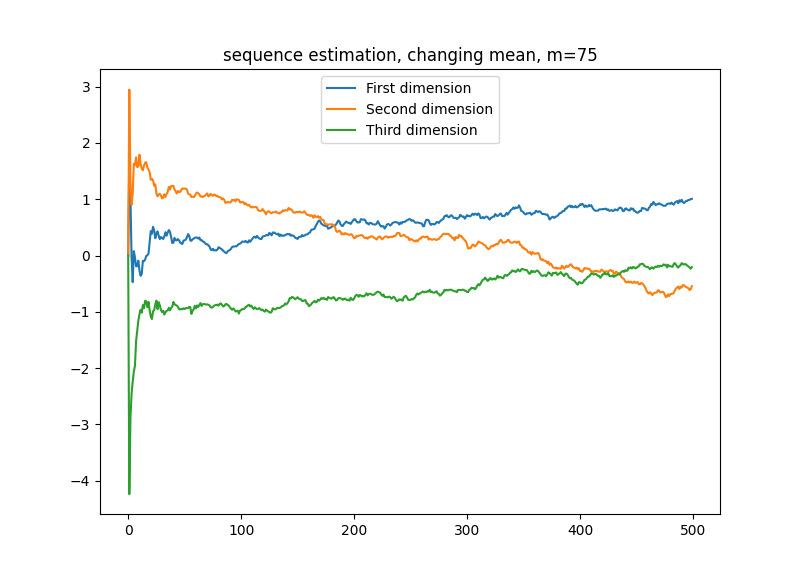
\includegraphics[width=0.75\textwidth]{03_sequential_estimation/indep_1_m75.png}
    \caption{Sequential estimation of a dataset with a changing mean.}
\end{figure}
\begin{figure}[h]
    \centering
    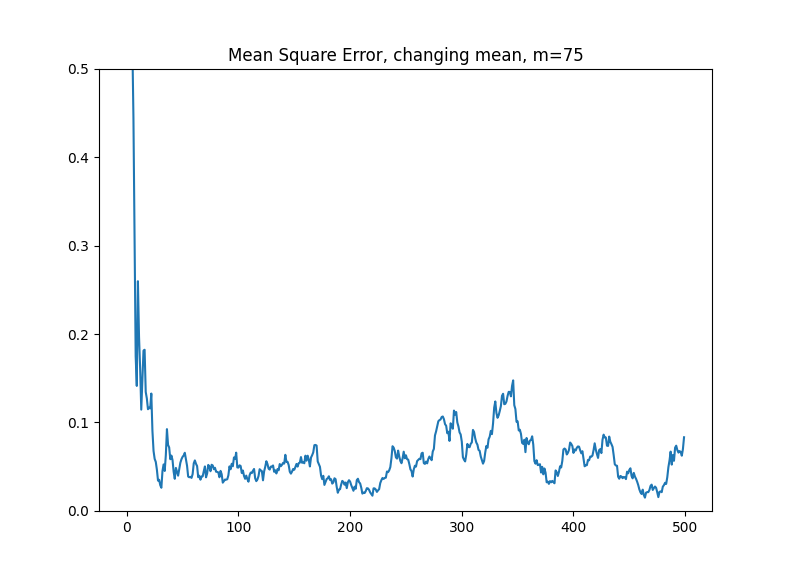
\includegraphics[width=0.75\textwidth]{03_sequential_estimation/indep_2_m75.png}
    \caption{Error of the above estimation.}
\end{figure}
\begin{figure}[h]
    \centering
    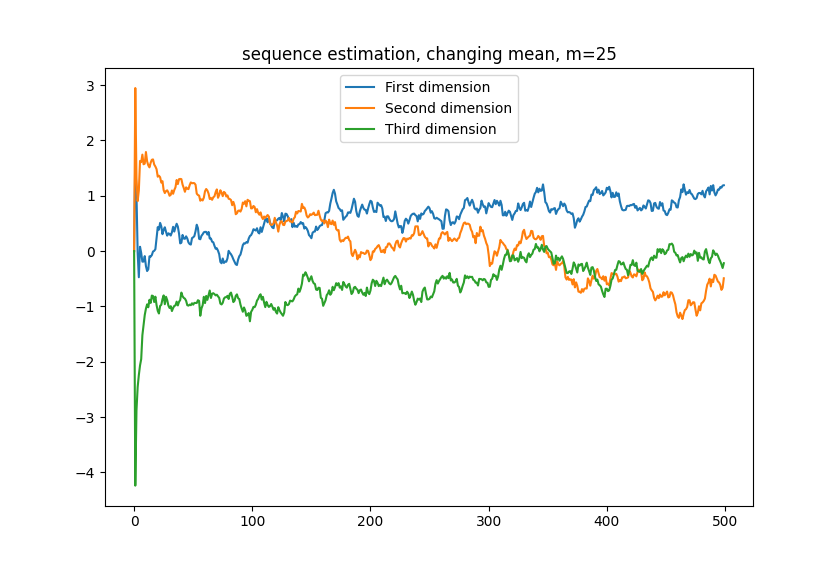
\includegraphics[width=0.75\textwidth]{03_sequential_estimation/indep_1_m25.png}
    \caption{Smaller M}
\end{figure}
\begin{figure}[h]
    \centering
    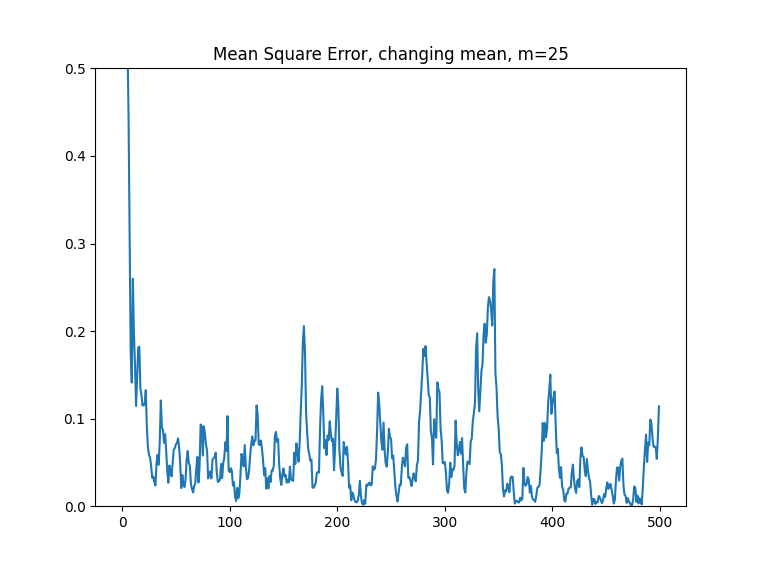
\includegraphics[width=0.75\textwidth]{03_sequential_estimation/indep_2_m25.png}
    \caption{Error of the above estimation.}
\end{figure}
\begin{figure}[h]
    \centering
    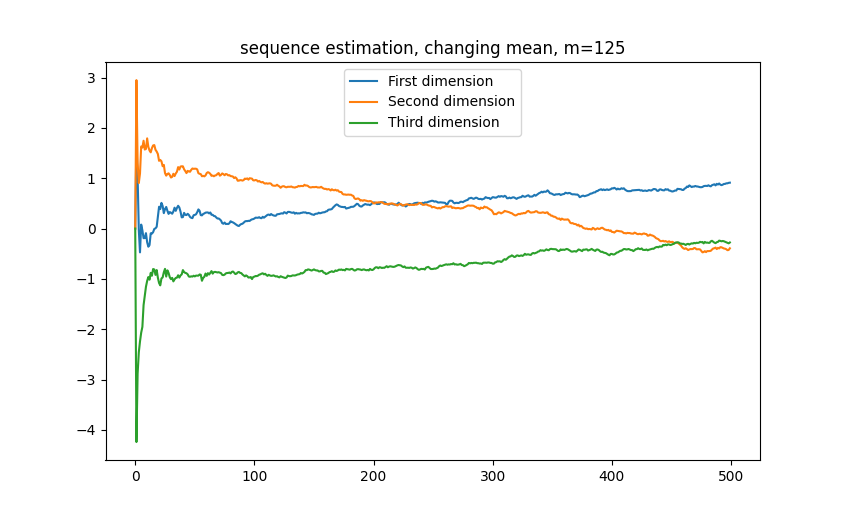
\includegraphics[width=0.75\textwidth]{03_sequential_estimation/indep_1_m125.png}
    \caption{Larger M}
\end{figure}
\begin{figure}[h]
    \centering
    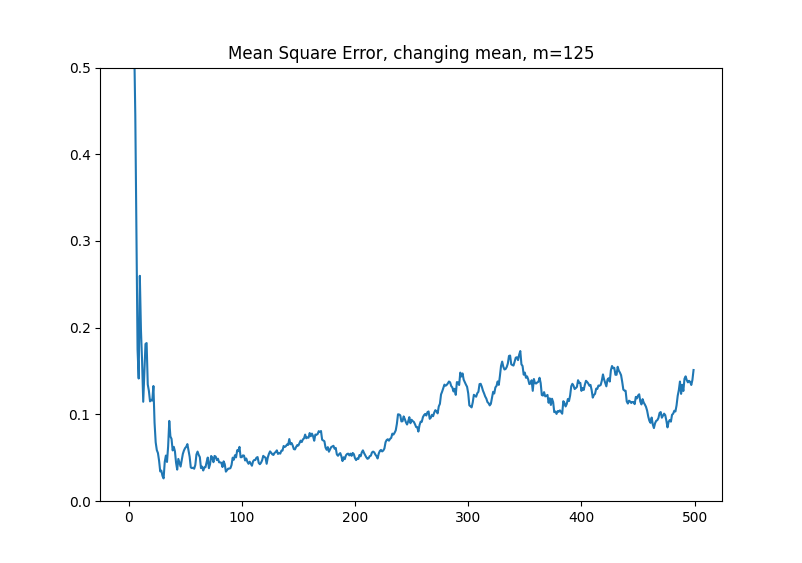
\includegraphics[width=0.75\textwidth]{03_sequential_estimation/indep_2_m125.png}
    \caption{Error of the above estimation.}
\end{figure}

\end{document}

